\newif\ifcommentenabled \commentenabledtrue
\newcommand{\TS}[1]{\ifcommentenabled\textcolor{red}{TS: #1}\fi}

\documentclass[12pt, a4paper, titlepage]{report}
\usepackage[dvipdfmx]{graphicx}
\usepackage[nottoc,numbib]{tocbibind}
\usepackage[utf8]{inputenc}
\usepackage{amsmath}
\usepackage{color}
\usepackage{enumerate}
\usepackage{hyperref}
\usepackage{mathptmx}
\usepackage{minted}
\usepackage{pdfpages}
\usepackage{tikz}
\usetikzlibrary{intersections, calc, arrows.meta}
\hypersetup{
  colorlinks = true,
  linkcolor = cyan
}

% Title Page
\title{Bachelor Thesis \\ TODO: TITLE}
\author{
  03190413 Takemaru Kadoi
  \\[1cm]
  {\small Supervisor: Prof. Masahiro Fujita},
  {\small Advisor: Assistant Prof. Taro Sekiyama}
  \\[1cm]
  {\small University of Tokyo, Department of Information and Communication Engineering}
}
\date{\today}

\begin{document}

% front page
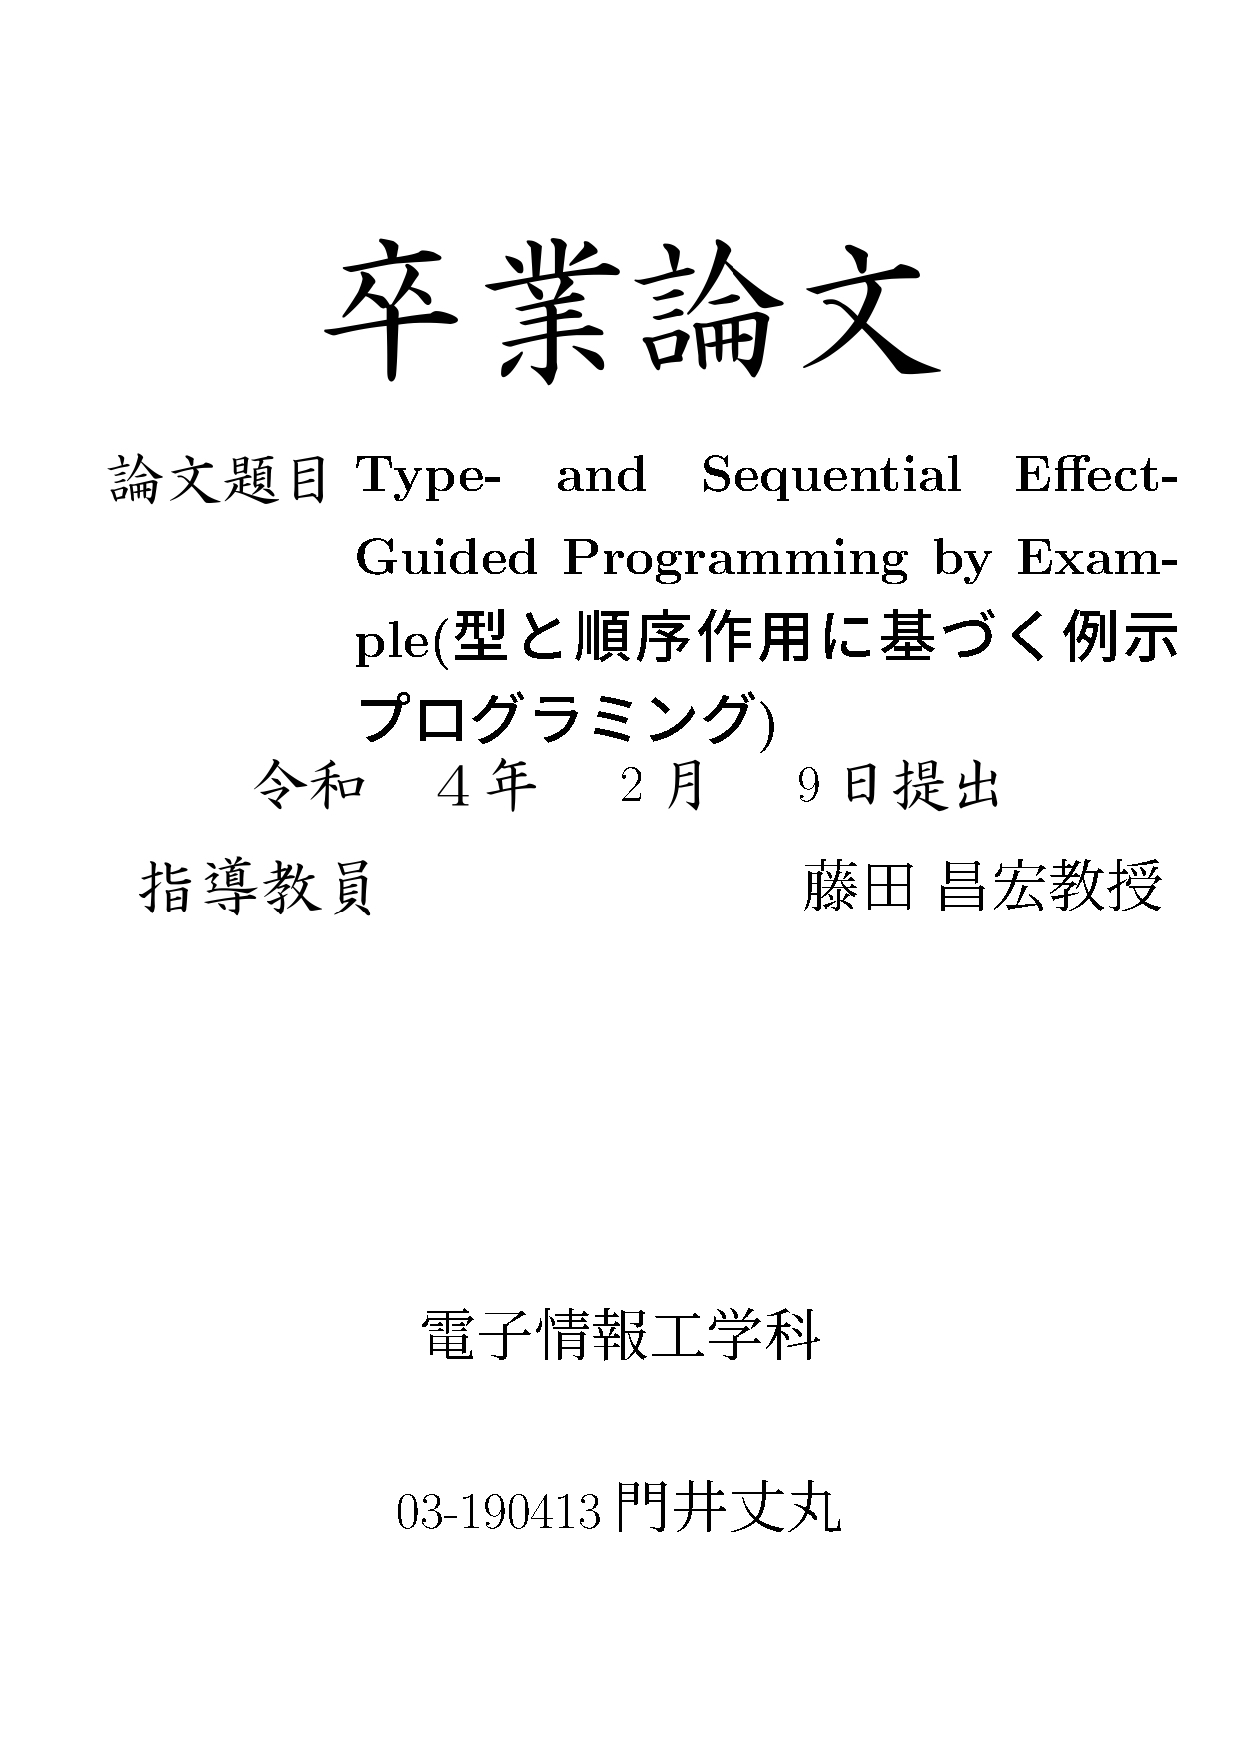
\includepdf[pages={-}]{images/sotsuronFront.pdf}

% header
\maketitle
\newpage
\tableofcontents
\newpage

\chapter*{Acknowledgment}
This research was supervised by Prof. Fujita at the University of Tokyo and supported by Assistant Prof. Sekiyama at National Institute of Technology. \\
I thank my colleagues at the University of Tokyo, Miyasaka-san, Koike-san, Yu-san, Nagasawa-san, and Yi-san.
% TODO: add twitter accounts
I also show my gratitude to my good friends, hnkz, Akio, Saeki, Arahata, Hori, Naito, Chen, and Sakura.

\chapter{Abstract} % overview of the research topic
\label{section:abstract}
Recently, increasing number of tools are made to enhance the productivity of programmers. One of the technologies that have contributed is program synthesis.
I discuss the motivation of this research and briefly explain what program synthesis is on chapter \ref{section:introduction}.
on chapter \ref{section:method}.
on chapter \ref{section:experiment}.
on chapter \ref{section:conclusion}.

\chapter{Introduction}
\label{section:introduction}
  \section{Motivation}
  \section{Program Synthesis}
    \cite{gulwani2017program}
  \section{Existing Methods}
  \section{Type and Effect System}
  \TS{This section may be unnecessary.}

\chapter{Method} % my approach to the problem
\label{section:method}
  \section{Syntax}
    \begin{minted}[breaklines, linenos]{ocaml}
      type 'a t = { name : string; mutable info : 'a};;
      let p = { name = "John"; info = 23 };;
      let double_quote = '"'
      let broken_highlight = ()
    \end{minted}
  \section{Semantics}
    \subsection{Static Semantics} % type-checking rules
    \subsection{Dynamic Semantics} % evaluation rules
  \section{Type and Effect System}
    \subsection{Type System}
    \subsection{Effect System}
  \section{Synthetic Process}

\chapter{Experiment} % quantitative result
\label{section:experiment}
\section{Result}
\section{Consideration}

\chapter{Conclusion} % qualitative result and future work
\label{section:conclusion}

\bibliographystyle{unsrt}
\bibliography{
  bib/synthesis
}

\end{document}
